\documentclass[]{elsarticle} %review=doublespace preprint=single 5p=2 column
%%% Begin My package additions %%%%%%%%%%%%%%%%%%%
\usepackage[hyphens]{url}

  \journal{Journal of Petroleum Science And Engineering} % Sets Journal name


\usepackage{lineno} % add
  \linenumbers % turns line numbering on
\providecommand{\tightlist}{%
  \setlength{\itemsep}{0pt}\setlength{\parskip}{0pt}}

\usepackage{graphicx}
\usepackage{booktabs} % book-quality tables
%%%%%%%%%%%%%%%% end my additions to header

\usepackage[T1]{fontenc}
\usepackage{lmodern}
\usepackage{amssymb,amsmath}
\usepackage{ifxetex,ifluatex}
\usepackage{fixltx2e} % provides \textsubscript
% use upquote if available, for straight quotes in verbatim environments
\IfFileExists{upquote.sty}{\usepackage{upquote}}{}
\ifnum 0\ifxetex 1\fi\ifluatex 1\fi=0 % if pdftex
  \usepackage[utf8]{inputenc}
\else % if luatex or xelatex
  \usepackage{fontspec}
  \ifxetex
    \usepackage{xltxtra,xunicode}
  \fi
  \defaultfontfeatures{Mapping=tex-text,Scale=MatchLowercase}
  \newcommand{\euro}{€}
\fi
% use microtype if available
\IfFileExists{microtype.sty}{\usepackage{microtype}}{}
\usepackage[margin=1in]{geometry}
\bibliographystyle{elsarticle-harv}
\usepackage{longtable}
\ifxetex
  \usepackage[setpagesize=false, % page size defined by xetex
              unicode=false, % unicode breaks when used with xetex
              xetex]{hyperref}
\else
  \usepackage[unicode=true]{hyperref}
\fi
\hypersetup{breaklinks=true,
            bookmarks=true,
            pdfauthor={},
            pdftitle={Bayesian Optimization: A New Sample Efficient Workflow for Reservoir Optimization under Uncertainty},
            colorlinks=false,
            urlcolor=blue,
            linkcolor=magenta,
            pdfborder={0 0 0}}
\urlstyle{same}  % don't use monospace font for urls

\setcounter{secnumdepth}{5}
% Pandoc toggle for numbering sections (defaults to be off)

% Pandoc citation processing
\newlength{\cslhangindent}
\setlength{\cslhangindent}{1.5em}
\newlength{\csllabelwidth}
\setlength{\csllabelwidth}{3em}
% for Pandoc 2.8 to 2.10.1
\newenvironment{cslreferences}%
  {}%
  {\par}
% For Pandoc 2.11+
\newenvironment{CSLReferences}[2] % #1 hanging-ident, #2 entry spacing
 {% don't indent paragraphs
  \setlength{\parindent}{0pt}
  % turn on hanging indent if param 1 is 1
  \ifodd #1 \everypar{\setlength{\hangindent}{\cslhangindent}}\ignorespaces\fi
  % set entry spacing
  \ifnum #2 > 0
  \setlength{\parskip}{#2\baselineskip}
  \fi
 }%
 {}
\usepackage{calc}
\newcommand{\CSLBlock}[1]{#1\hfill\break}
\newcommand{\CSLLeftMargin}[1]{\parbox[t]{\csllabelwidth}{#1}}
\newcommand{\CSLRightInline}[1]{\parbox[t]{\linewidth - \csllabelwidth}{#1}\break}
\newcommand{\CSLIndent}[1]{\hspace{\cslhangindent}#1}

% Pandoc header
\usepackage{setspace}
\usepackage{booktabs}
\usepackage{longtable}
\usepackage{array}
\usepackage{multirow}
\usepackage{wrapfig}
\usepackage{float}
\usepackage{colortbl}
\usepackage{pdflscape}
\usepackage{tabu}
\usepackage{threeparttable}
\usepackage{threeparttablex}
\usepackage[normalem]{ulem}
\usepackage{makecell}
\usepackage{xcolor}



\begin{document}
\begin{frontmatter}

  \title{Bayesian Optimization: A New Sample Efficient Workflow for Reservoir Optimization under Uncertainty}
    \author[a]{Peyman Kor\corref{1}}
  
    \author[a]{Aojie Hong}
  
    \author[a]{Reidar Brumer Bratvold}
  
      \address[a]{Energy Resources Department, University of Stavanger, Stavanger, Norway}
      \cortext[1]{Corresponding Author, peyman.kor@uis.no}
  
  \begin{abstract}
  \doublespacing An underlying challenge in well-control optimization during field development is that flow simulation of a 3D, full physics grid-based model is computationally prohibitive. In a robust optimization setting, where flow simulation has to be repeated over a hundred(s) of geological realizations, performing a proper optimization workflow becomes impractical in many real-world cases. In this work, to alleviate this computational burden, a new sample-efficient optimization method is presented. In this context, sample efficiency means that the workflow needs a minimum number of forward model evaluations (flow-simulation in the case of reservoir optimization) while still being able to capture the global optimum of the objective function. Moreover, the workflow is appropriate for cases where precise analytical expression of the objective function is nonexistent. Such situations typically arise when the objective function is computed as the result of solving a large number of PDE(s), such as in reservoir-flow simulation. In this workflow, referred to as ``Bayesian Optimization'\,' the objective function for samples of decision variables is first computed using a proper design experiment. Then, a Gaussian Process (GP) is trained to mimic the surface of the objective function as a surrogate model. While balancing the exploration-exploitation dilemma, a new decision variable is queried from the surrogate model and a flow simulation is run for this query point. Later, the output of the flow-simulation is assimilated back to the surrogate model which is updated given the new data point. This process continues sequentially until termination criteria are reached. To validate the workflow and get better insight into the details of optimization steps, we first optimize a 1D problem. Then, the workflow is implemented for a 3D synthetic reservoir model in order to perform robust optimization in a realistic field scenario. Finally, a comparison of the workflow with two other commonly used algorithms in the literature, namely Particle Swarm Intelligence (PSO) and Genetic Algorithm (GA) is performed. The comparison shows that the workflow presented here will reach the same near-optimal solution achieved with GA and PSO, yet reduce computational time of the optimization 5X (times). We conclude that the method presented here significantly speeds up the optimization process leveraging a faster workflow for real-world 3D optimization tasks, potentially reducing CPU times by days or months, yet gives robust results that lead to a near-optimal solution.
  \end{abstract}
   \begin{keyword} Optimization, Gaussian Process, Probabilistic Modeling, Bayesian\end{keyword}
 \end{frontmatter}

\newpage

\hypertarget{introduction}{%
\section{Introduction:}\label{introduction}}

\doublespacing

Well control optimization (also known as production optimization) can be defined as making the best decision for a set of control variables in continuous space, given a pre-defined objective function. The objective function generally relies on a reservoir simulator to evaluate the proposed well control decision for the period of the reservoir life cycle. On the other hand, the control decisions are usually well injection/production rates or bottom-hole pressure (BHPs). Given the objective function and alternatives, uncertainties are represented by a set of geological realizations (i.e., an ensemble). Known, as Robust Optimization (RO), within RO, the objective is to find a control vector to maximize the expected value of the objective function over geological uncertainty in contrast to deterministic case, where the sources of uncertainty in geological model is ignored. Well control optimization typically poses challenges as the objective function is non-linear and non-convex. Moreover, the optimization problem becomes computationally demanding in the RO setting as many geological models must be considered. This renders the optimization computationally expensive, if not prohibitive, in large-scale systems where (potentially) hundreds of wells are involved.

Literature of well control optimization can be viewed from two angles. At first, the focus is on the type of optimization algorithm used for this type of problem. Broadly speaking, the type of optimization algorithm could be divided into two categories, gradient-based and gradient-free.

(Sarma et al., 2005) applied adjoint-gradient based optimization to waterflooding problem. (van Essen et al., 2009) optimized hydrocarbon production under geological uncertainty (in RO setting), where an adjoint-based method is used for obtaining the gradient information. The adjoint-based procedure is more efficient because it uses gradients that are constructed efficiently from the underlying simulator. However, the adjoint-based method requires access to the source code of the reservoir simulator, which is seldom available for commercial simulators, and it is computationally intensive. Chen et al. (2009) introduced the ensemble-based optimization method (EnOpt), in which the gradient is approximated by the covariance between the objective function values and the control variables. Do and Reynolds (2013) analyzed the theoretical connections between EnOpt and other approximate gradient-based optimization methods. Having realized that it is unnecessary to approximate the ensemble mean to the sample mean as was done by Chen et al. (2009), Do and Reynolds (2013) used the ensemble mean in their EnOpt formulation. Stordal et al. (2016) had a theoretical look at EnOpt formulation and showed that EnOpt is a special case of well-defined natural evolution strategy known as Gaussian Mutation. It is a special case from this perspective that EnOpt is Gaussian Mutation without the evolution of covariance matrix \((\sum)\) of multivariate Gaussian density.

On the other hand, gradient-free methods represent a useful alternative when gradients are not available or are too expensive to compute. It can be divided into two major classes, stochastic and pattern search; these methods are noninvasive with respect to the simulator, though they are usually less efficient and require a larger number of function evaluations than adjoint-gradient methods.

Probably the first use of the gradient-free method for subsurface application, (Harding et al., 1998) applied genetic algorithm (GA) to production scheduling of linked oil and gas fields. A Comparison study was performed, and they showed the GA outperforms simulated annealing (SA) and sequential quadratic programming (SQP) techniques, and a hybrid of the two. GA was utilized later by (Almeida et al., 2007) for the optimization of control valves in the intelligent wells. They found that significant profit was achieved in comparison to using conventional methods (no valve control). More recently, (Lushpeev and Margarit, 2018) applied Particle Swarm Optimization (PSO) to a real field case to find optimum injection mode for the mature field. Control variables were the change in injection rates of 3 injectors, and results of field experiments show the improvement in relative recovery after applying the modified solution of the optimization algorithm.

Generalized Pattern-search (GPS) methods (Dennis, n.d.; Torczon, 1997) are another types of gradient-free techniques has been applied in well control optimization problem. The pattern-search method relies on polling; a stencil is centered at the current solution at any particular iteration. The stencil comprises a set of directions such that at least one is a descent direction. If some of the points in the stencil represent an improvement in the objective function, the stencil is moved to one of these new solutions. GPS, including its variant (Mesh Adaptive Direct Search), is usually considered a local search method, but due to its ability to parallelize, it has been well used in the literature of well control optimization. (Asadollahi et al., 2014; Echeverría Ciaurri et al., 2010; Foroud and Seifi, 2016; Nwachukwu et al., 2018). To overcome the locality of the GPS methods, hybrid of the PSO as global method and then using pattern search for local search in iterative (PSO-MADS) way as well proposed in the work of (de Brito and Durlofsky, 2020; Isebor et al., 2013).

\hypertarget{survey-of-surrogate-based-papers-in-onepetro-database}{%
\subsection{Survey of surrogate-based papers in Onepetro database}\label{survey-of-surrogate-based-papers-in-onepetro-database}}

In the previous section, we reviewed commonly used optimization algorithms in well control optimization. However, it should be noted that even with a more efficient optimization method like EnOpt, still performing full RO optimization with full physic reservoir simulators is computationally prohibitive (we will discuss the detail of this computational burden more in Section 2) (Hong et al., 2017). In order to make RO feasible, two general approaches have been introduced. The first set of techniques targets the flow problem. These methods include capacitance-resistance models (Hong et al., 2017; Yousef, 2006; Zhao et al., 2015), deep-learning and machine learning surrogates (Chai et al., 2021; Kim et al., 2020; Kim and Durlofsky, 2021; Nwachukwu et al., 2018) and reduced-physics simulations (de Brito and Durlofsky, 2020; Møyner et al., 2014; Nasir et al., 2021). These methods generally entail approximating the high-fidelity flow simulation model with a lower-fidelity or reduced order model, or a model based on simplified flow physics. To get insight into how this line of research is evolving, we performed a small text mining task. Mining the more than 100000 peer-reviewed papers published in (www.onepetro.org), we count the number of the papers with ``one'' of the following keywords in their abstract:

\begin{enumerate}
\def\labelenumi{\arabic{enumi}.}
\tightlist
\item
  ``Proxy'' + '' Optimization'' + ``Reservoir''
\item
  ``Surrogate'' + ``Optimization'' + '' Reservoir''
\item
  ``Reduced-physics model'' + ``Optimization'' + '' Reservoir''
\end{enumerate}

The period of 1995-2020 was considered. As Figure \ref{fig:onepetroanalysis} reveals, we see that just around ten years ago in this research area we had around \textasciitilde{} 10 papers per year, now that number is around three times more. Part of this interest in developing a ``physic-reduced model'' could be attributed to development in machine learning research and transferring knowledge for building data-driven models for subsurface applications.

\begin{figure}

{\centering 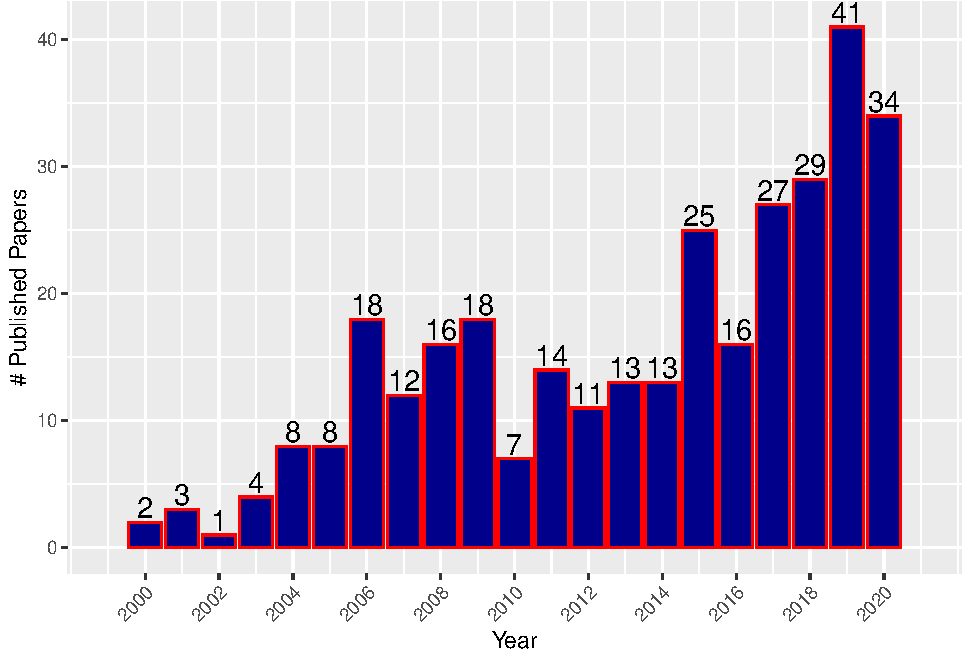
\includegraphics[width=468px]{0_Paper1_main_files/figure-latex/onepetroanalysis-1} 

}

\caption{Counting the number of papers with the keyword in their abstract vs year}\label{fig:onepetroanalysis}
\end{figure}

In this work, we propose Bayesian Optimization (BO). We will show that BO, as a gradient-free method, has characteristics of the global optimization method in escaping local optima or saddle area. While, at the same time, the workflow overcomes the typical downside of gradient-free methods, which is need for many function evaluations. Due to utilizing the probabilistic model to mimic the expensive objective function, BO workflow is inherently efficient, meaning that a minimum number of function evaluations is needed to achieve a near-optimum solution. To validate this idea, we compared the BO with two other gradient-free, global optimization techniques (PSO, GA) while showing BO reaches similar (same) solutions while using only 20\% of function evaluations, compared to the other two algorithms. We would like to refer to the results of the ``OLYMPUS Optimization Benchmark Challenge'' (Fonseca et al., 2020) where the gradient-free methods showed the best performance in achieving the highest NPV, but participants mentioned the pain of these methods as they carry huge computational burden due to large function evaluation (Chang et al., 2020; Pinto et al., 2020; Silva et al., 2020). In light of benchmark results, bringing the efficiency to the gradient-free optimization category is a significant contribution, presented in this work.

In Section 2 (``Problem Statement''), we will describe the underlying problem in well control optimization and the need for efficient optimization to deal with the enormous computational burden of optimization. In Section 3 (``Bayesian Optimization Workflow''), we will lay out the mathematical background of the BO workflow. In section 4, ``Examples Cases,'' BO workflow is applied to two numerical cases. The first one is a 1-D example where we guide our audience with a step-by-step process about applying BO. The second numerical example is the field case. Where BO is applied to a 3-D synthetic geological model for optimizing injection scheme in eight injectors. In section 5, ``Comparison with other Alternatives,'' a comparison of the BO with two global optimization techniques, PSO and GA, is presented. The paper ends with ``Concluding Remarks'' in section 6.

\newpage

\hypertarget{problem-statement}{%
\section{Problem Statement}\label{problem-statement}}

In general, an optimization task can be defined as a search process for the maximum output value of a ``well behaved''\footnote{In this context, it means the function is defined everywhere inside the input domain, it is single-valued and continuous.} objective function \(f\). Can be defined as \(f: \chi \rightarrow \mathbb{R}\) where acceptable solutions \(\chi\), has a dimension of \(D\), \(\chi \subseteq \mathbb{R}^D\) :

\begin{equation}
\begin{aligned}
& \underset{x}{\text{maximize}}
& & f(x) \\
& \text{subject to}
& & x \subseteq \chi
\end{aligned}
\label{eq:globalopt}
\end{equation}

In Figure \ref{fig:optglobal} we can see some examples where the surface of \(f\) could be challenging to be optimized. The surfaces on the left side need careful attention to avoid getting stuck in local optima. Figures on the right side show presence of saddle area, where the gradient of function \(f\) is zero, in some cases in only one direction, possibly all directions. In this work, the focus is on the type of objective function \(f\), which is challenging to optimize because of the following three difficulties:

\begin{itemize}
\tightlist
\item
  \(f\) is explicitly unknown. This is a typical case in reservoir optimization problems where the Net Present Value (NPV) or Recovery Factor (RF) is computed through solving a vast number of partial differential equations through flow simulation. Thus, a precise analytical expression for the objective function is not available, avoiding the applicability of techniques that exploit the analytical expression of the objective function.
\item
  The surface of \(f\) is multi-modal. Meaning that \(f\) is non-convex in the domain of \(\chi\) , and the optimization algorithm must visit all local optima to find the ``global'' one.
\item
  Most importantly, forward evaluation of \(f\) is computationally expensive. This point will be discussed more in detail below.
\end{itemize}

\begin{figure}

{\centering 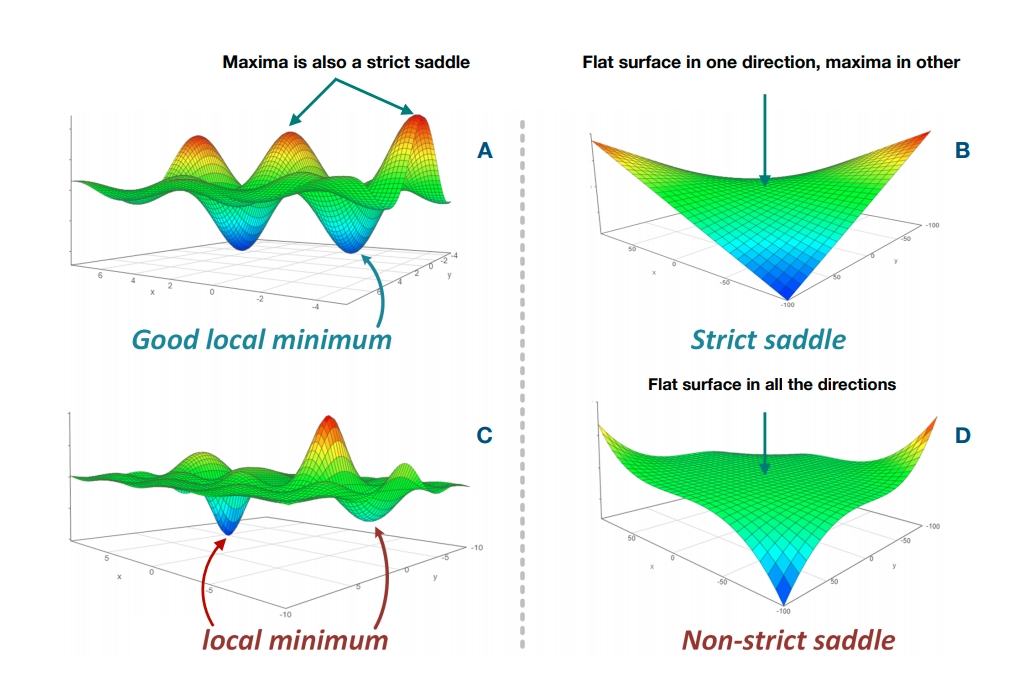
\includegraphics[width=0.7\linewidth]{img/globalopt} 

}

\caption{This plot may change, it does not show what exactly I want to say...}\label{fig:optglobal}
\end{figure}

In the examples of this paper, the goal is to maximize the subsurface-outcomes-based NPV (in USD). Thus, the primary objective function is also referred to as simply NPV in the rest of this paper. This objective function has been widely used in both well control and field development optimization studies. In a deterministic setting, the uncertainty in the geological parameters is disregarded and the optimization is performed based on a single geological model. Therefore, in the case of deterministic optimization, the objective function can be defined as:

\begin{equation}
J(\mathbf{u, G})= \sum_{k=1}^{K} \Bigg [\sum_{j=1}^{N_p}p_oq_{o,j,k}(\mathbf{u, G}) 
- \sum_{j=1}^{N_p}p_{wp}q_{wp,j,k}(\mathbf{u, G}) - 
\sum_{j=1}^{N_{wi}}p_{wi}q_{wi,j,k}(\mathbf{u, G}) \Bigg]\frac{\Delta t_k}{(1+b)^{\frac{t_k}{D}}}
\label{eq:npvdet}
\end{equation}

Where the first term in the double summation corresponds to the oil revenue; the second term is water-production cost and third term corresponds to the water-injection cost. Equation \eqref{eq:npvdet} is considered as objective function in the deterministic setting since only a single geological model is considered. The \(G\) in the Equation \eqref{eq:npvdet} is ``the geological model.'' The additional parameters in the Equation are as follows: \(K\) is the total number of timesteps; \(N_p\) is the total number of production wells subject to optimization; \(N_{wi}\) is the total number of water-injection wells subject to optimization; \(k\) is the timestep index; \(j\) is the well-number index; \(p_o\) is the revenue from oil production per unit volume (in USD/bbl); \(p_{wp}\) is the water-production cost per unit volume (in USD/bbl); \(p_{wi}\) is the water-injection cost per unit volume (in USD/bbl); \(q_o\) is the oil-production rate (in B/D); \(q_{wp}\) is the water-production rate (in B/D); \(q_{wi}\) is the water-injection rate (in B/D); \(\Delta t_k\) is the time interval for timestep \(k\) (in days); \(b\) is the discount rate (dimensionless); \(t_k\) is the cumulative time for discounting; and D is the reference time for discounting (\(D = 365\) days if b is expressed as a fraction per year and the cash flow is discounted daily). \(\mathbf{u}\) in Equation \eqref{eq:npvdet} is the control vector (i.e., a vector of control variables) defined as \(\mathbf{u} = [u_1, u_2, \cdots, u_N]^D\), where \(D\) is the number of control variables (dimension of optimization problem).

As mentioned above, Equation \eqref{eq:npvdet} lacks to capture the uncertainty in the geological model. In contrast, in a Robust Optimization (RO) setting, the objective is to optimize the expected value over all geological realizations (assumption here is decision maker is risk-neutral). The objective function for the RO setting then can be defined as: (in the case of equiprobable geological realization)

\begin{equation}
\overline{J}(\mathbf{u}) = \frac{\sum_{re=1}^{n_e} J(\mathbf{u,G_{re}})}{n_e}
\label{eq:npvopt}
\end{equation}

Where in Equation \eqref{eq:npvopt} contrary to Equation \eqref{eq:npvdet}, there is not one, rather \(n_e\) geological realizations, each of them written as \(G_{re}\). In this work, the objective is to optimize the Equation \eqref{eq:npvopt}, where it is simply EV value of NPV defined in \eqref{eq:npvdet} over all realizations.\\

It is well defined in the literature that optimizing Equation \eqref{eq:npvopt} is computationally prohibitive (de Brito and Durlofsky, 2021; Hong et al., 2017; Nwachukwu et al., 2018). Not only because thousand(s) of PDE have to be solved in the flow-simulation in order to compute the \(q_o, q_{wp}, q_{wi}\); the flow simulation must be enumerated over all realizations \(n_e\) to compute \(\overline{J}(u)\). Let's assume a simple case to illustrate the computational burden of this optimization problem. Assume that an E\&P enterprise is in the process of finding the bottom hole pressure of five injection wells and shut-in time of other five production wells, \(D=10\). The geology team of the enterprise comes up with 100 geological realizations of the model.(\(n_e=100\)). Now, if we suppose that the reservoir model is 3D with a moderate number of grid cells, it is not hard to imagine that flow-simulation of a fine grid model will take \textasciitilde1hr. Then, simply having 100 realizations means that each forward computation of \(\overline{J}(u)\) takes around \textasciitilde100 hr. Considering that the enterprise has to decide in 6 month period (in the best case, it can be interpreted as 6 months CPU running time), which means that a total number of the available budget for running the forward model is\(\frac{6 \times 30 \times 24 }{100}= 43.2 \approx 50\) is around 50. The budget of only \(50\) forward model in ten-dimensional, non-linear, and non-convex optimization problem is relatively low. To put this in simple terms, if we say that each dimension of the control variable \(\mathbf{u}\), could be discretized into ten possible cases, then total available solutions for this optimization problem will be \(\text {Number of all possible solutions} = 10^{10}\). As it is clear, finding the best solution from a pool of ten billion possible solutions with only 50 shots is a pretty much hard undertaking.\\

The rest of this paper will be arguing that the Bayesian Optimization workflow is well suited to deal with the three difficulties described above. Where the workflow needs to capture the optimum global point (area) while having a small forward evaluation budget.

\newpage

\hypertarget{bayesian-optimization-workflow}{%
\section{Bayesian Optimization Workflow}\label{bayesian-optimization-workflow}}

\hypertarget{overall-view}{%
\subsection{Overall View}\label{overall-view}}

Bayesian Optimization (BO) is an optimization method that builds a probabilistic model to mimic an expensive objection function. The probabilistic model is build based on a finite number of function evaluations. These finite number of evaluations is done as initialization of the workflow and build a probabilistic model.

After initialization and building a probabilistic model, at each iteration, a new query point is evaluated using the the expensive objective function, then the new data \((u,f(u))\) is assimilated back to probabilistic model to update the model.The unique methodology of using a non-deterministic surrogate model makes Bayesian optimization (BO) an efficient global optimizer capable of both decision space exploration and exploitation.

\hypertarget{gaussian-process}{%
\subsection{Gaussian Process}\label{gaussian-process}}

In this work, we employ the widely used Gaussian process (GP) as the probabilistic model. Known also as surrogate model (since it tries to mimic the real, expensive objective function), GPs are attractive because they are computationally traceable with capability to quantity the the uncertainty of interest (Murphy, 2022; Rasmussen and Williams, 2006). A Gaussian process can be seen as an extension of the Gaussian distribution to the functional space. Key Assumption in (GP) is that: the function values at a set of \(M > 0\) inputs, \(\mathbf{J} = [J({u_1}), ...,J(u_M)]\), is jointly Gaussian, with mean and Covariance defined as:

Note: Here we use the objective function described in previous section with the notation \(\overline{J}(\mathbf{u})\), where \(\mathbf{u}\) is control variables. However, just for simplicity in notation, we drop the bar sign and write objective function with \(J(\mathbf{u})\).

\begin{equation}
  \begin{split}
& \mathbf{\mu(u)} = [\mu(u_1),\cdots,\mu(u_M)] \\
& \text{Cov}(J(\mathbf{u}),J(\mathbf{u'}))= \kappa(\mathbf{u},\mathbf{u'})
  \end{split}
\label{eq:mean_cov}
\end{equation}

\[\mathbb{E}[J(\mathbf{u})] = \mu(\mathbf{u})\] \[ \text{Cov} [J(\mathbf{u}),J(\mathbf{u'})]= \kappa(\mathbf{u},\mathbf{u'})\]

where \(\mathbf{\mu(u)}\) is a mean function and \(\kappa(\mathbf{u},\mathbf{u'})\) is a covariance function (or kernel). \(\kappa(\mathbf{u},\mathbf{u'})\)being specifies the similarity between two values of a function evaluated on \(\mathbf{u}\), and \(\mathbf{u'}\) . A GP is a distribution over functions completely defined by its mean covariance function as:

\begin{equation}
J(\mathbf{u}) \sim \mathcal{N}(\mathbf{\mu(u)}, \kappa(u,u'))
\label{eq:mean_cov_gp}
\end{equation}

\[J(\mathbf{u}) \sim \mathcal{N}(\mathbf{\mu(u)}, \kappa(u,u'))\]

where \$\textbackslash mathcal\{N\}\$ denotes the multivariate normal distribution. For simplicity we assume the prior mean function to be zero: \(\mu(\mathbf{u}) = 0\). This assumption is not restrictive because as more training points are observed the prior is updated and becomes more informative. As was discussed in (Shahriari et al., 2016) there many choice for the covariance function, most commonly used ones in the literature has been depicted in the \ref{tab:cov-tab}.

\begin{table}[H]

\caption{\label{tab:cov-table} Several types of covariance function for the GP process}
\centering
\begin{tabu} to \linewidth {>{\raggedright}X>{\raggedright}X}
\toprule
Covariance Kernels & assumeing $h=||x-x'||$\\
\midrule
Gaussain & $\Large \kappa (u,u') =\sigma_f^2 exp(-\frac{h^2}{2\ell^2})$\\
Matern $\mu=\frac{5}{2}$ & $\Large \kappa (u,u') =\sigma_f^2(1 + \frac{\sqrt{5}|h|}{\ell}\frac{5h^2}{3\ell^2})exp(-\frac{ -\sqrt{5}|h|}{\ell})$\\
Matern $\mu=\frac{3}{2}$ & $\Large \kappa (u,u') =\sigma_f^2(1 + \frac{\sqrt{3}|h|}{\ell})exp(-\frac{-\sqrt{3}|h|}{\ell})$\\
Exponetial & $\Large \kappa (u,u') =\sigma_f^2 exp(-\frac{|h|}{\ell})$\\
Power-Exponetial & $\Large \kappa (u,u') =\sigma_f^2 exp(-(\frac{|h|}{\ell})^p)$\\
\bottomrule
\end{tabu}
\end{table}

Where in the table, \(\ell\) is lengthscale, and \(h\) is eludian distance of \(u\), \(u'\) (\(|h|^2=(u-u')^\intercal(u-u')\)). Given \(N\) observations of the objective function \(J(u)\) at points \(x_i\), the complete covariance/kernel matrix is given by:

Assuming we start GP with finite number of initial evaluation of \(J(u)\) in the data set of \(\mathcal{D}=(\mathbf{u}_n,\mathbf{J}(\mathbf{u}_n): n=1:N)\) where \(J(u_n)\) is the noise-free observation of the function evaluated at \(u_n\).

Now we consider the case of predicting the outputs for new inputs that may not be in \(\mathcal{D}\). Specifically, given a test set (prediction set) set \(U_*\) of size \(N_* \times D\), we want to predict the function outputs \(J^* = [J(u_1),\cdots, J(x_{N_*})]\). By definition of the GP, the joint distribution \(p(\mathbf{J}_{X}, \mathbf{J}_*| \mathbf{X}, \mathbf{X_*})\) has the following form:

\begin{equation}
\begin{bmatrix}  {\bf {J}_U}  \\  {{\bf J}_*} \end{bmatrix} \sim \mathcal{N} \begin{pmatrix} \begin{bmatrix}  {{\bf \mu}_U}  \\  {{\bf \mu}_*} \end{bmatrix},\begin{bmatrix} {{\bf K}_{U,U}}  & {{\bf
K}_{U,*}}  \\  {{\bf \mathbf{K}^\intercal}_{U,*}} & {{\bf K}_{*,*} } \end{bmatrix}\end{pmatrix}
\label{eq:gp-model-mat}
\end{equation}

Where,\(\mathbf{\mu}_U\) prior knolwdge about mean value of \(\mathbf{J}(U)\), defined as \(\mathbf{\mu}_U=[m(u_1),\cdots,m(u_N)]\). The \emph{Gram} matrix, \(K_{XX}\), is \(N \times N\) matrix, with each element is covariance of \(\mathbf{u}\) and \(\mathbf{u'}\):

\begin{equation}
\left (
\begin{array}{ccc}
\begin{array}{l}
\kappa(\mathbf{u_1},\mathbf{u_2})
\end{array}
& \cdots & 
\begin{array}{l}
\kappa(\mathbf{u_1},\mathbf{u_N})
\end{array} \\
\vdots & \ddots & \vdots\\
\begin{array}{l}
\kappa(\mathbf{u_N},\mathbf{u_1})
\end{array} &
\cdots & 
\begin{array}{l}
\kappa(\mathbf{u_N},\mathbf{u_N})
\end{array} 
\end{array}
\right )
\label{eq:kernel_struct}
\end{equation}

\[K_{U,U}=\kappa({\mathbf{U},\mathbf{U}})\left (
\begin{array}{ccc}
\begin{array}{l}
\kappa(\mathbf{u_1},\mathbf{u_2})
\end{array}
& \cdots & 
\begin{array}{l}
\kappa(\mathbf{u_1},\mathbf{u_N})
\end{array} \\
\vdots & \ddots & \vdots\\
\begin{array}{l}
\kappa(\mathbf{u_N},\mathbf{u_1})
\end{array} &
\cdots & 
\begin{array}{l}
\kappa(\mathbf{u_N},\mathbf{u_N})
\end{array} 
\end{array}
\right )\]

By the standard rules for conditioning mutivariate gaussain distribution,we can drive the posterior (conditional distribution of \(\mathbf{J}(U_*)\) given the \(\mathcal{D}=(\mathbf{U},\mathbf{J}(U)\)) in closed form as following:

\begin{align*}
  \begin{split}
p(\mathbf{J}_*|\mathbf{U_*,\mathcal{D})}= & \:  \mathcal{N}(\mathbf{J_*| \mathbf{\mu_*},\textstyle \sum_{\ast}}) \\
{\mathbf{\mu_\ast}}= & \:  m(\mathbf{U_\ast}) +\mathbf{K}^\intercal_{U,*} \mathbf{K}^{-1}_{U,U}(\mathbf{J}_U-m(\mathbf{U})) \\
\textstyle \sum_{\ast}=& \:  \normalsize{\mathbf{K}_{\ast,\ast}-\mathbf{K}^\intercal_{U,\ast}\mathbf{K}_{U,U}^{-1}\mathbf{K}_{U,\ast}}
  \end{split}
\label{eq:post_mean_cov}
\end{align*}

\hypertarget{step.3-deciding-on-next-bfxast-based-on-posterior}{%
\subsubsection{\texorpdfstring{Step.3 Deciding on next \(\bf{x}^\ast\) based on Posterior}{Step.3 Deciding on next \textbackslash bf\{x\}\^{}\textbackslash ast based on Posterior}}\label{step.3-deciding-on-next-bfxast-based-on-posterior}}

Posterior of the probalistic model quantify the uncertainty over the space of the unknown function, \(f\). The question is what is the next \(\mathbf{u}^\ast\) to be sampled from the \emph{expensive function}? One could select the next point arbitrarily but that would be wasteful.

To answer this question, we define an utility function and the next query point is the point which has the maximum utility. The literature of BO have seen many utility function (called acquisition function in the computer science community). These include the Improvement based policies (Probability of Improvement (PI), Expected Improvement(EI)), optimistic policies (Upper Confidence Bound (UCB)) or Information-based (like Thompson Sampling (TS)). The full review of these utility function an their strengthen and weakness could be reviewed in (Shahriari et al., 2016).

In Expected Improvement (EI) policy choose the next query point as the one which has the highest expected improvement over the space of the \emph{expensive function}

\begin{equation}

utility(u;\theta,\mathcal{D})=\alpha_{EI}=\int_{y}^{}max(0,\mathbf{J}(u_*)-f)p(\mathbf{J}(\mathbf{u_*})|\mathcal{D}) \,dy

\label{eq:uti_int}

\end{equation}

\[utility(\mathbf{u}_*;\theta,\mathcal{D})=\alpha_{EI}=\int_{y}^{}max(0,\mathbf{J}(\mathbf{u}_*)-f)p(\mathbf{J}(\mathbf{u_*})|\mathcal{D}) \,dy\]

However, we do not have access to the \emph{expensive function}, \(f\), therefore we replace the \(f\) with the best available solution found so far, \(\mathbf{J}^+\) . We would like to note that \(\mathbf{u}_*\) is

\begin{eqution}

utility(u;\theta,\mathcal{D})=\alpha_{EI}=\int_{y}^{}max(0,\mathbf{J}(u_*)-\mathbf{J}^+)p(\mathbf{J}(\mathbf{u_*})|\mathcal{D}) \,dy

\label{eq:uti_int_2}

\end{equation}

\[utility(u;\theta,\mathcal{D})=\alpha_{EI}=\int_{y}^{}max(0,\mathbf{J}(u_*)-\mathbf{J}^+)p(\mathbf{J}(\mathbf{u_*})|\mathcal{D}) \,dy\]

\newpage

\hypertarget{example-cases}{%
\section{Example Cases}\label{example-cases}}

\hypertarget{d-toy-problem}{%
\subsection{1-D toy Problem}\label{d-toy-problem}}

In this section, a 1-D toy problem is considered to illkuystrate the Bayes Optimization workflow dicussed in the previous section. The 1-D problem was selected sinnce it will help to visuluze all the steps of the workslow making easier explanation of the concepts. Though, it it can bee senn from the next section, the workflow can easily extened to to higer dimetional problem. The \emph{True function} to be optimized in this section has an analytical expression as, given the box constrains:

\begin{equation}
\begin{aligned}
& \underset{x}{\text{maximize}}
& & f(x) = 1-\frac{1}{2}(\frac{\sin (12x)}{1+x} + 2\cos(7x)x^5 + 0.7)  \\
& \text{subject to}
& & 0 \leq x \leq 1
\end{aligned}
\label{eq:1deq}
\end{equation}

Since the analytical expression of function available and being 1-D problem, the global optimum of the function had been found at the \(x_M = 3.90\). The plot of the function and the optimum point has been shown in the Figure \ref{fig:onedplot}

\begin{figure}

{\centering 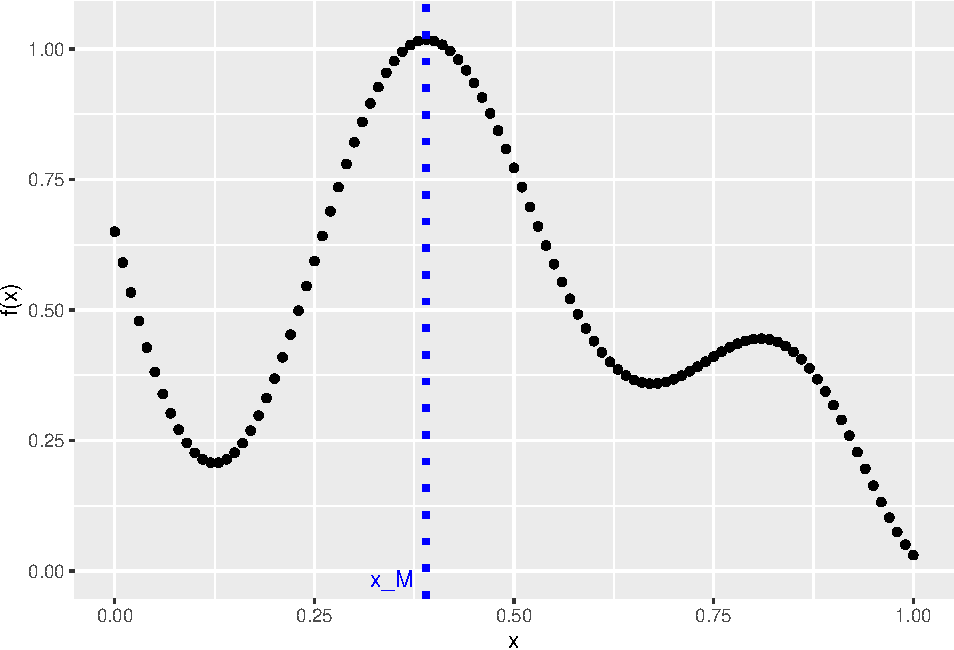
\includegraphics[width=0.9\linewidth]{0_Paper1_main_files/figure-latex/onedplot-1} 

}

\caption{Plot of 1-D equation with blue dash line representing the global optimum}\label{fig:onedplot}
\end{figure}

However, it is worth to mention that the analytical expression of objective function in many of real world problems are not avilable, what is avilable is a \emph{samples} from the objective function. Thefore, in the coming example a few samples are sequentiall drawn from the objective function to resemble the real case scenario. However, we know the global optimum of the objective function in hindsight, just in the case we want to copare the performace of Bayesian optimisation algorithem.

Thefore, as Figure \ref{fig:exampleshow}, the 5 sample points, \(x=[0.05,0.2,0.5,0.6,0.95]\) were selected as the initialization of the workflow. In the upper plot, blue lines represnets the samples from posterior of the gaussian model conditioned on the five sample points. The grey area represents the 95\% confidence interval while the red curve represents the mean value of the samples (blue lines). The first point to infer from the Figure \ref{fig:exampleshow} is there no uncertainty on the sample point. As shown, there is no grey zone on sample point since as was dicussed in the previous section, here we consider the ``noise-free'' observation. Also, worth to mention that we have wide more uncertainity (wider grey band) in the reas that are more distant from the observation, simply meaning we are less uncertain close to observation points. on the ``extrpolation,'' meaning in the ares outseide of the observation points, the probalistic model shows inetrsting behaviour. on those ``exterme'' area, the mean curve tend to move toward the mean of all observation points , here around 0, showing the model refelctes the mean-revervion behaviour when it comes extrpolation.

The lower part of Figure \ref{fig:exampleshow}, shows the plot of utility function at each x values. Worth to note that as the plot suggest, the utility(\(\alpha_{EI}\)) function will have the muti-modal structure, meaning in the optimization process multi-start gradient method will be helpful, in order to avoid stock in the local optima. In this work, as was explained in the preious section, the multi-start gradient method was used. The blue dotted line line shows the the \(x_{next}\) which is the point where the utility function, is maximum. Then this \(x_{next}\) is qured from the real function, and the the pair of \((x_{next}, f(x_{next}))\) is added to the intial data set, \(\mathcal{D}\). Going back to the lower figure at Figure \ref{fig:exampleshow}, the utility has two mode around point \(x=0.5\), say \(x_{0.5}^+\) and \(x_{0.5}^-\), however the point \(x_{0.5}^-\) is selected as the next query point. Readers can be rfereed to the upper plot and it is clear that there is more uncertainity around point \(x_{0.5}^-\) than \(x_{0.5}^+\) which given the form of utility function, that is understandable. The utility function always looking for the point that not only maximize the mean value, but also intereded in the points that has higher variannce, which is the case between two points \(x_{0.5}^+\) and \(x_{0.5}^-\).

\begin{figure}

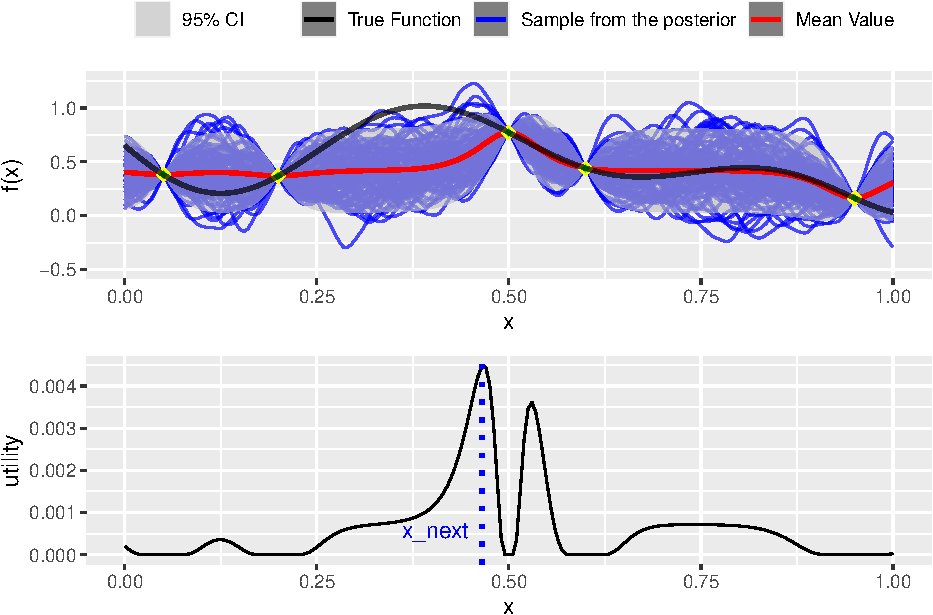
\includegraphics[width=1\linewidth,height=0.75\textheight]{0_Paper1_main_files/figure-latex/exampleshow-1} \hfill{}

\caption{Ite1 - Top: Gaussian posterior over the initial sample points; Lower: Utility function over the x values}\label{fig:exampleshow}
\end{figure}

Calling the Figure \ref{fig:exampleshow} as the iteration \# 1, now we can start sampling sequentially. In the Figure \ref{fig:allinone} another two iteration has been provided. Wher in each row, the plot on the left represents the posterior on the gaussian condistioning, the right show the utility function. Note that in the Figure \ref{fig:allinone} all axis labels and legned were not included, to have better visibity. (more info about each plot can ben found in \ref{fig:exampleshow}) . Interesting to see tat in this example case, at the irteration \#2, the workflow query the point \(x=0.385\) which presents the best point so far found through BayesOpt workflow. Thefiore, after just two iteration we are around \(\frac{x_{best}}{x_{M}}=\frac{0.385}{0.390}=98.7%
\) of the global optima. Although this is case for 1-D problem, it is clearly showing the stength of the workflow to approach the lglobal optima, in as few as possible iteration. In this case after iteration\#2, tyhe total number of tim,e that the real function has been quered is \(\text{size}(\mathcal{D}) + \text{size}(total iteration) = 5 + 2=7\) .

\begin{figure}

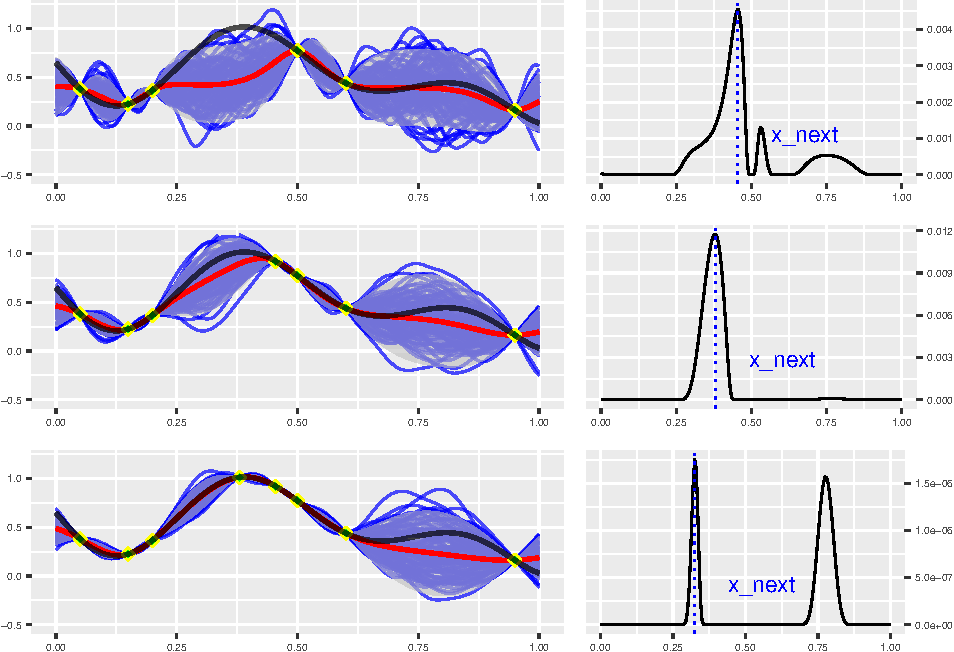
\includegraphics[width=0.9\linewidth,height=0.9\textheight]{0_Paper1_main_files/figure-latex/allinone-1} \hfill{}

\caption{Gaussian posterior of over the initial sample points}\label{fig:allinone}
\end{figure}

Before going to apply the same workflow at the field scale, the 1-D example presented here offer another useful feature of the Bayesian Optimisation. Looking at \ref{fig:allinone}, we can see that the maximum of utility function is at the iteration \# 3 in order of \(10^{-6}\) . That show that after optimization, eve best point to be queried in the next section has a very little utility. So can safely stop the process, since querying points to be sampled from the expensive function has a negligible potential to improve our search in optimization.

\newpage

\hypertarget{field-scale}{%
\subsection{Field Scale}\label{field-scale}}

\hypertarget{synthetic-3d-reservoir-model}{%
\subsubsection{Synthetic 3D Reservoir Model}\label{synthetic-3d-reservoir-model}}

In this section, the BayesOpt workflow is applied to the synthetic 3D reservoir model. The trough introduction of the model and gelogical describtion can be found in (Jansen et al., 2014) . Known as ``Egg Model'' it has a geology of channelized depositional system.

\begin{figure}

{\centering 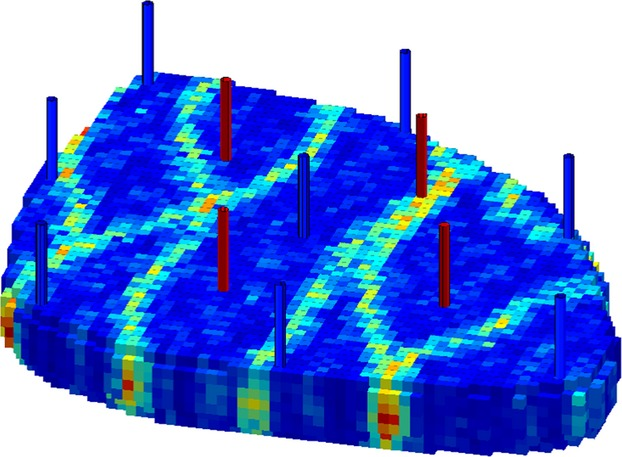
\includegraphics[width=300px]{img/egg_base} 

}

\caption{Well locations in Egg model, blue ones are injection, the red producers}\label{fig:eggbase}
\end{figure}

The 3D model has eight water injectors and four producers wells shown in Figure \ref{fig:eggbase}. The has a geological realizations of patterns of highly permeable channels which are described by 100 equi-probable geological realizations, three of which are illustrated in left side of Figure \ref{fig:combine}.(Hong et al., 2017).

Relative permeabilities and the associated fractional flow curve of the model have shown in right side of Figure \ref{fig:combine} .All the wells are vertical and completed in all seven layers. Capillary pressure is ignored. The reservoir rock is assumed to be incompressible. The model has a life-cycle of 10 years. Here, the injection rate to be maiintaned over life-cycle of reservoir is going to be optimized. Thus, given eight injection wellls, the optimizatijon workflow has the eight dimnetions.However, the optimization in not unbounded, the water can be adjusted from 0 to 100 m3/day, making the box-constrain optimization. The injectors are operated with no pressure constraint, and the producers are under a minimal BHP of 395 bars without rate constraint.

\begin{figure}

{\centering 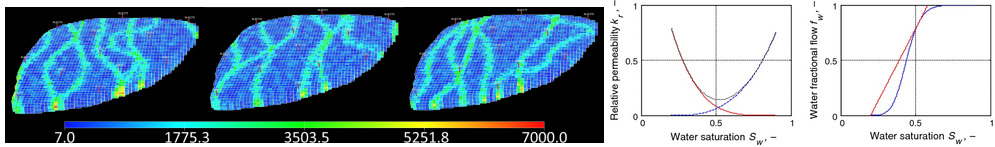
\includegraphics[width=1\linewidth]{img/combine} 

}

\caption{Left: Three geological realizations of the 3D model; Right: Rel perm and fractional flow curve}\label{fig:combine}
\end{figure}

\hypertarget{well-control-optimization}{%
\subsubsection{Well Control Optimization}\label{well-control-optimization}}

Reviewing the equation raised in the section 3, here the goal is robust optimization of the field , given geological realizations as follow:

\begin{equation}
\text{Objective Func(u)}= \overline{J}(u) = \frac{\sum_{i=1}^{n_e} J_r(u,G_i)}{n_e}  \label{eq:npvoptrep}
\end{equation}

Equation \eqref{eq:npvoptrep}

\(u\) is Injection rate for the each injection well, therefore the control vector, to be optimizaed in this case is defined as:

\begin{equation}
u=[u_{inj1},u_{inj2},u_{inj3},u_{inj4},u_{inj5},u_{inj6},u_{inj7},u_{inj8}]^{\intercal} 
\label{eq:cont-vec}
\end{equation}

As the \eqref{eq:npvoptrep} suggest, the \(\overline{J}(u)\) need some parameters to be defined. The oil price (\(P_o\)), water production cost (\(p_{wp}\)) and water injection cost (\(P_{wi}\)) in \(dollar/m^3\) has been provided in the Table \ref{tab:npvparam}. Also, in this work the cash flow is disconted daily and the discount factor is avilable in the \ref{tab:npvparam}. We would like to note that in this work due to avoid further computional burden in optimization process, 10 realizations of the egg model has been considered, therefore \(n_e=10\) in Equation \eqref{eq:npvoptrep}.

\begin{table}[H]

\caption{\label{tab:npvparam}Required Parameters needed for calculation of Expected NPV}
\centering
\begin{tabu} to \linewidth {>{\raggedright}X>{\raggedright}X>{\raggedright}X>{\raggedright}X}
\hline
Item & Pric & Items & Value\\
\hline
P\_o & 315 & b & 8\%\\
\hline
P\_wp & 47.5 & D & 365\\
\hline
P\_wi & 12.5 & n\_e & 10\\
\hline
\end{tabu}
\end{table}

\hypertarget{bayesopt-workflow}{%
\subsubsection{BayesOpt Workflow}\label{bayesopt-workflow}}

As it was discussed, the starting point of the BAyesOpt workflow is to randomly sample the initial data pairs \(\mathcal{D}\) which is used to build the Gaussian model of the response surface to the input variables. In this work, forty samples fom the Latin hyper cube sampling (LHS) method were drawn. The LHS is prefred in this work to Monte Carlo since it provides the stratifcation of the CDF of each variable, leading to better coverage of the input variable space. The Figure \ref{fig:lhssampling} show the results of the \(\overline{J}(u)\) for each sample from LHS. Also, The maximum \(\overline{J}(u)\) found from sampling has been shown with blue line. Setting the specific seed number (since LHS is in itself is random process), we get the max \(NPV\) aciehved here was \(35.65 \$MM\). Looking at Figure \ref{fig:lhssampling} it is worth to mention that random sampling like the LHS is not helpful to consistently approach the global optimum point, and there is a need for efficient workflow to find the optimum point while using the a few as possible sampling from real function.

\begin{figure}

{\centering 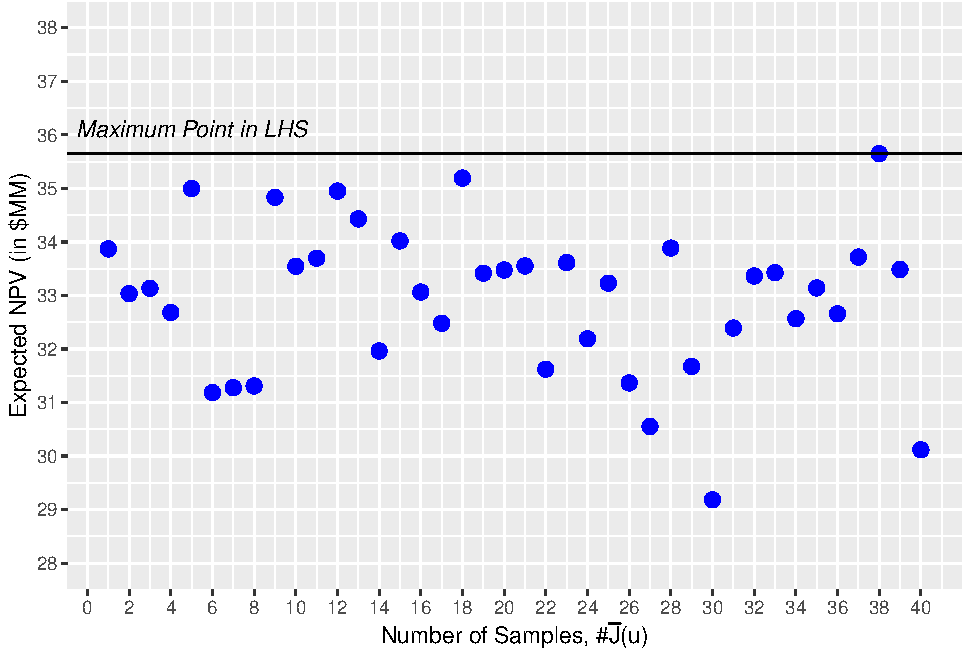
\includegraphics[width=468px]{0_Paper1_main_files/figure-latex/lhssampling-1} 

}

\caption{Expected NPV as result of forty sampling from LHS}\label{fig:lhssampling}
\end{figure}

Having the initial data found through LHS, we can build the probalistic model of the reposnse surface and sequentially sample from the \emph{expensive-to-evaluate} function. Unfortunately, win this section we can not plot the posterior of the probalistic model, condition on the above forty LHS samples, due being the space is eight-dimetional, and hard to visulize. The Figure \ref{fig:lhsbayesop} shows the expected NPV found after ten sequential sampling resulted from the BayesOpt workflow. Readers are refreed to this point that in the figure, not all red points are increasing and some points are lower than previous points. The reason for this behaviour is the nature of BayesOpt algorith. We can suggest that in the points that has lower expected NPV from the previous, we may reached the lower optimum point, but those points helped us to decrease the uncertainity, which is helpful for the further sampling. We can see that after just ten evaluation of the expenside function (here it means finding the expected NPv from running 10 geological realization using flow simulation) we reach the new record Expeted NPV of \(max \overline{J}(u)=36.85\)\(\$MM\).

\begin{figure}

{\centering 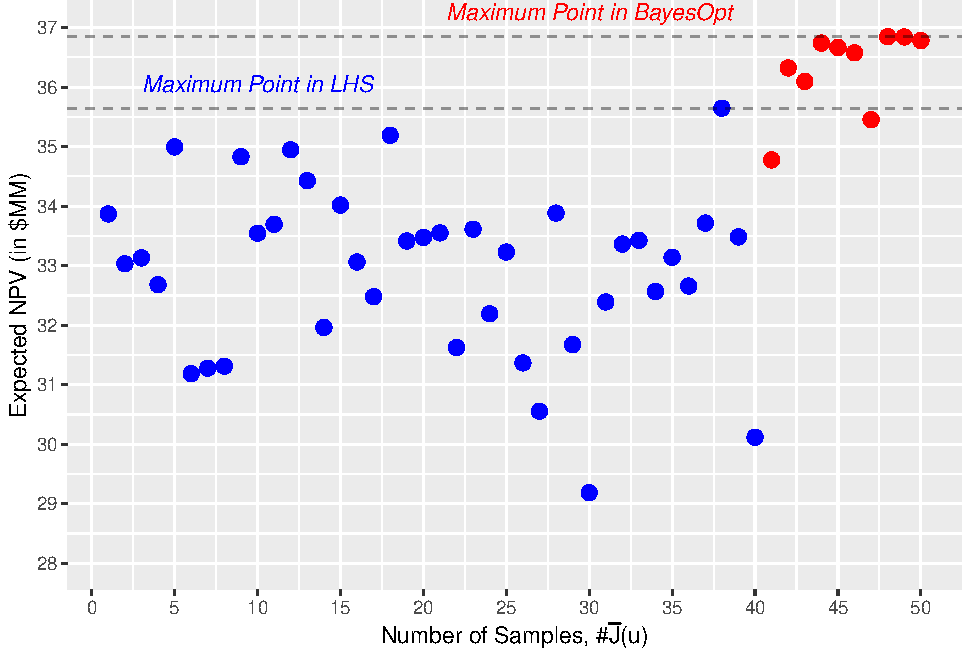
\includegraphics[width=468px]{0_Paper1_main_files/figure-latex/lhsbayesop-1} 

}

\caption{Blue points represnts the sample from LHS, red points represents the samples from the BayesOpt Workflow}\label{fig:lhsbayesop}
\end{figure}

Now, as we explained in the 1-D section, the plot of the utility at each iteration could provide some useful information about the optimization process. The Figure \ref{fig:utilitycurve} plots the \(\alpha_{EI}^*(\mathcal{D}, \theta^*)\) (Equation \eqref{eq:exp-easy} )versus the ten iteration in this work. In fact the notaion \(\alpha_{EI}^*\) means the optimum of the \(\alpha_{EI}(u;\mathcal{D},\theta^*)\) after running multi-start (1000)- L-BFGS-B on all \(u\) values. Now, we can see that in the figure the \(\alpha_{EI}^*\) is decreasing going toward the zero. It can be inferred from this trend that, we are going out of the \emph{good} \(u\) values to be sampled from the expensive function, can be intepreted that we are in the vicinity of global optima, if we see after several iteration still \(\alpha_{EI}^*\) is less than \(10^-6\).

\begin{figure}

{\centering 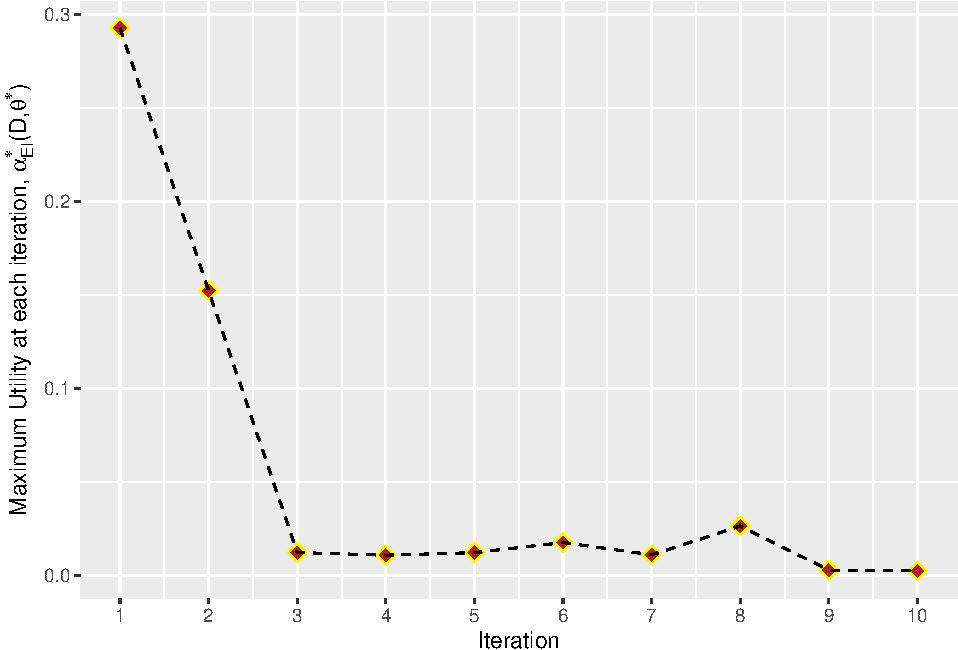
\includegraphics[width=468px]{0_Paper1_main_files/figure-latex/utilitycurve-1} 

}

\caption{Maximum utility at each iteration, after running L-BFGS-B to find the u with max utility, $\alpha_{EI}^*$}\label{fig:utilitycurve}
\end{figure}

Given that the BayesOpt inherintely has stochasric natrae ( from this perspective that having thje diffrenet initialization in LHS sampling will affect the final solution), in this section BayesOpt is repeated with diffret initilization. Ideally, this repeation shouwl be conducted 100 or 1000 times, to get better overview of the convergence of the algorithm given diffrent initilization. Though, because of the computional burden, in this work only three repeations were performed. optimization Repeat the Optimization, three times, in different initial design points. Figure \ref{fig:difinit} shows results of three repeations. At each repeation (top, middle, bottom), the blue dots come from diffrente seed numbers and they are diffrente. Then, gicen that initialization \(\mathcal{D}\), sequential sampling from the expenive function is perfomred, shown in the red points. Like previous case, in these repeations, 40 samples drawn from LHS algortihem, the 10 were taken thorigh BAyesOpt lagorith, totaling 50 samples. At each row of the Figure \ref{fig:difinit}, two horizontal lines show the maximum point \(\overline{NPV}\) in both random sampling phase (LHS) and BayesOpt phase. As it can be noted from the Figure \ref{fig:difinit}, at each repeation, the BayesOpt will improve the solution with small sample evaluation of the \(\overline{J}(u)\). Thefore, improvemnet following the BayesOpt phase indepned of the initial design, yet the bigger question is whether given different initial design, the algorithm converge the vicinity of global optima. What is refered here is that if having different initilaization will lead completely different final solution, that hints that the algorithm has a ``local'' search, in conrast, if the solutions leads to one specif close \(u^*\), that reprsents that algorithm have a ``global'' view on the surface of the objective function. In the case of ``global'' optimization having diferent initilizatin should lead to simular final solution, since the algorithm will not get stuck in local optimum points, close to initilalized data. This is common practice in the gradient-based optimization where the algorithm is powerfull in local optimization and in order to avoid stuck in local exterme points, ``multi-start'' runs are performed in order to search the global point in the objective function.

\begin{figure}

{\centering 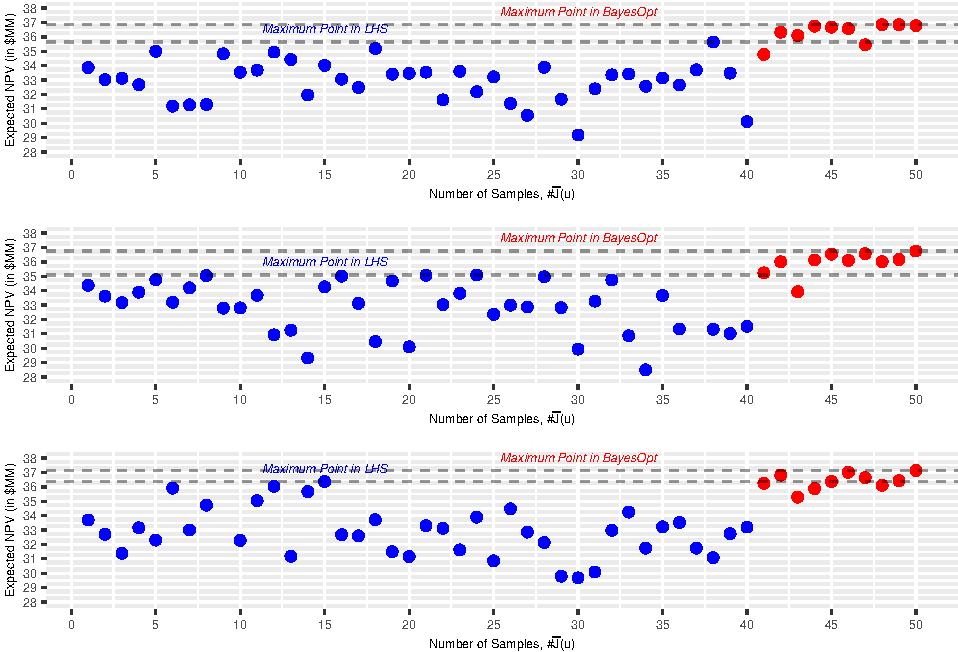
\includegraphics[width=0.9\linewidth,height=0.9\textheight]{0_Paper1_main_files/figure-latex/difinit-1} 

}

\caption{BayesOpt workflow applied to Syntetic 3D model, in three different initialization}\label{fig:difinit}
\end{figure}

To further continue thiss dicussion on the effect of initialization on the final solution, the \(u^*\) value for each repeatation has been show on the left side of Figure \ref{fig:diffu}. Where the \(u^*\) is the vector of 8 dimention, each value shows the optimum injection rate for the 10 years life cycle of the field, in \(m^3/D\). We woul like to note that the y axis was plotted from the range of 5 to 100. The reason for this is to show that in this optimization problem, injection of each wells can take any number between 5\(m^3/D\) to 100 \(m^3/D\), and the y axis shows the full extend of the value optimum zation worlkflow can reach. Visually, looking at the left plot at Figure \ref{fig:diffu}, we can see that the final solution of three repeations at each weels, does not differ significantly from each other . With small exception of (injection \#2), it seems all the final solutions converges to the same solution. This feature that can be loosly said as ``robustness'' of optimization workflow to initial design is very helpfu, from this sense that we do not neeed to resetart the optimization with different initilaization, since they all will converges to the similar solution. From this perspective, authours can infere that BayesOpt workflow can be considered as ``global'' optimization method, as it shows the workflow avoids stuck in local exterme pointsor saddle regions. The plot on the left side of Figure \ref{fig:diffu} shows that mean injection rate (mean of three repeations) and erro bar at each injection wells. The bottom of error bar in this plot shows the \(mean-sd\) and top of bar is \(mean + sd\) . As we can see that we do not see significant variation in the final solution in each repeations, also the plots recoomnds that in the case of repeating the optimization with more than three times (like 10 or 100), it can lead to lower variation in final solution.

\begin{figure}

{\centering 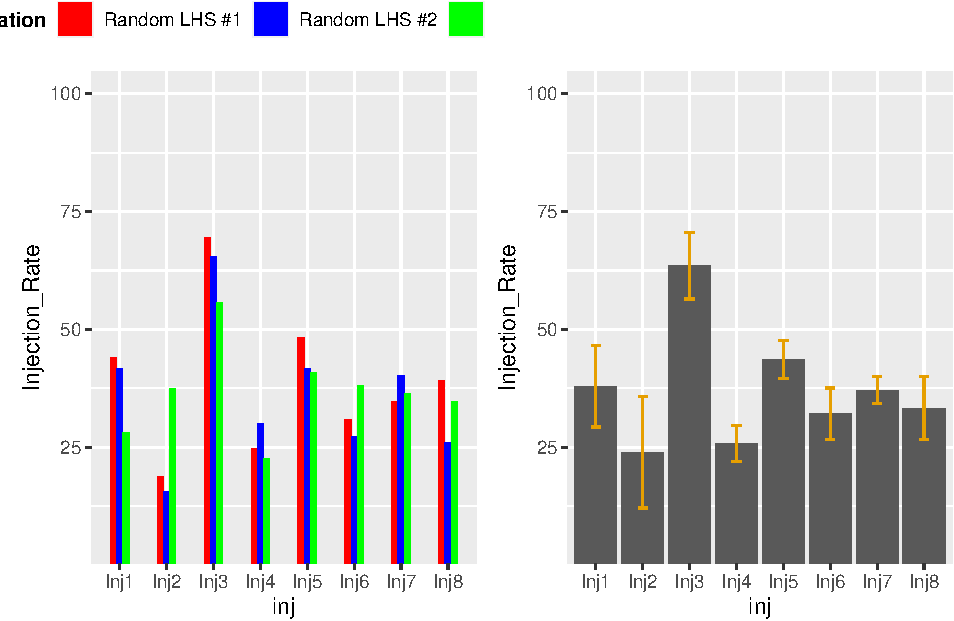
\includegraphics[width=0.9\linewidth]{0_Paper1_main_files/figure-latex/diffu-1} 

}

\caption{Left: final solution of optimization algorithm in three different initialization, Right: Mean and error bar of each injection rate at each injection wells}\label{fig:diffu}
\end{figure}

\newpage

\newpage

\hypertarget{bayesopt-performance-versus-other-alternatives}{%
\section{BayesOpt performance versus other alternatives}\label{bayesopt-performance-versus-other-alternatives}}

In this section the aim is to compare the performance of the Bayesopt workflow with other available optimization algorithm commonly used for reservoir optimization under uncertainty. The literature of field development optimization enjoys wide varieties of the workflow and algorithm applied to field development. Broadly speaking those can be divided into two categories adjoint-gradient and derivative-free. Adjoint methods, such as those described in (Forouzanfar and Reynolds, 2014; Li and Jafarpour, 2012; Volkov and Bellout, 2018) can provide computational advantage in terms of efficiency. They are, however, local methods, and it is known that broad (global) searches can be advantageous in field development optimization methods.(de Brito and Durlofsky, 2021) - Therefore, in this work two well-know Derivative-free optimization (DFO) methods, extensively used reservoir optimization, named Genetic Algorithm (GA) (Chai et al., 2021; Holland, 1992) and Particle Swarm Optimization (PSO) (Eberhart and Kennedy, 1995; Jesmani et al., 2016) have been considered. In this section we provide a brief overview of each methods, but interested readers are refereed to the original papers.(Eberhart and Kennedy, 1995; Holland, 1992)

\hypertarget{particle-swarm-optimization-pso}{%
\subsection{Particle Swarm Optimization (PSO)}\label{particle-swarm-optimization-pso}}

PSO is a global stochastic search technique that operates based on analogies to the behaviors of swarms/flocks of living organisms. Originally developed by (Eberhart and Kennedy, 1995) , Considering a swarm with \(P\) particles, there is a position vector \(X_{i}^{t}=(x_{i1},x_{i2}, x_{i3},x_{in})^T\) and a velocity vector \(V^t_i=(v_{i1},v_{i2},v_{i3},v_{in})^T\) at a \(t\) iteration for each one of the \(i\) particle that composes it. These vectors are updated through the dimension \(j\) according to the following equations:

\begin{equation}
V^{t+1}_{ij} = \omega V^{t}_{ij} + c_{1}r_{1}^{t}(pbest_{ij}-X_{ij}^t) + c_2r_2^t(gbest_j-X_{ij}^{t})
\label{eq:pso}
\end{equation}

where \(i=1,2,..., P\) and \(j =1,2,...,n\). Equation \eqref{eq:pso} explains that there are three different contributions to a particle's movement in an iteration. In the first term, the parameter \(\omega\) is the inertia weight constant. In the second term, The parameter \(c_1\) is a positive constant and it is an individual-cognition parameter, and it weighs the importance of particle's own previous experiences. The other parameter second term is \(r_1^t\), and this is a random value parameter with {[}0,1{]} range. The third term is the social learning one. Because of it, all particles in the swarm are able to share the information of the best point achieved regardless of which particle had found it, for example, \(gbestj\). Its format is just like the second term, the one regarding the individual learning. Thus, the difference \((gbest_j - X^t_{ij})\) acts as an attraction for the particles to the best point until found at some t iteration. Similarly, \(c_2\) is a social learning parameter, and it weighs the importance of the global learning of the swarm. And \(r_2\) plays exactly the same role as \(r_1\). Where Equation \eqref{eq:psoup} updates the particle's positions. (Almeida and Leite, 2019)

\begin{equation}
X_{ij}^{t+1} = X_{ij}^{t} + V_{ij}^{t+1}
\label{eq:psoup}
\end{equation}

\hypertarget{genetic-algorithm-ga}{%
\subsection{Genetic Algorithm (GA)}\label{genetic-algorithm-ga}}

Genetic algorithm is a stochastic search algorithms that use evolutionary strategies inspired by the basic principles of biological evolution. First developed by John Holland (Holland, 1975) and his collaborators in the 1960s and 1970s, later has been applied for optimization and search problems Goldberg and Holland (1988); Mitchell (1998). The evolution process is as follow: GA starts with the generation of an initial random population of size \(P\), so for step \(k = 0\) we may write \({\theta_1^{(0)}; \theta_2^{(0)},\cdots, \theta_p^{(0)}}\), (step 1). The fitness of each member of the population at any step \(k\), \(f(\theta_i^{(k)})\), is computed and probabilities \(p_i^{(k)}\) are assigned to each individual in the population, usually proportional to their fitness, (step 2). The reproducing population is formed \textbf{selection} by drawing with replacement a sample where each individual has probability of surviving equal to \(p_i^{(k)}\), (step 3). A new population \({\theta_1^{(k+1)}; \theta_2^{(k+1)},\cdots, \theta_p^{(k+1)}}\) is formed from the reproducing population using crossover and mutation operators, step (4). Then, set \(k = k + 1\) and the algorithm returns to the fitness evaluation step, (back to step 2). When convergence criteria are met the evolution stops, and the algorithm deliver as the optimum (Scrucca, 2013).

\hypertarget{comparison-in-fixed-reservoir-simulation-budget-n50}{%
\subsection{Comparison in Fixed Reservoir Simulation Budget (N=50)}\label{comparison-in-fixed-reservoir-simulation-budget-n50}}

In first part of the comparison, we compare the Bayesopt with PSO and GA in fixed \(\overline{J}(u)\). It means that optimization process could continue, until they use \(\overline{J}(u)=50\) function evaluations. It is worth to mention that in fact \(\overline{J}(u)=50\) is equal to \(500\) reservoir simulations, due to number of realization, \(n_e=10\) and ten computation per each \(\overline{J}(u)\). Another point is parameters of PSO and GA. These two methods needs parameters to be defined by the user. In GA, these parameters are: Population Size, probability of crossover between pairs of chromosomes, probability of mutation in a parent chromosome, The number of best fitness individuals to survive at each generation. For PSO, the algorithm parameters are as below: size of the swarm, the local exploration constant, the global exploration constant.

\begin{table}

\caption{\label{tab:unnamed-chunk-9}Parameters of GA and PSO Methods}
\centering
\begin{tabu} to \linewidth {>{\raggedright}X>{\raggedright}X}
\toprule
parameters & value\\
\midrule
\addlinespace[0.3em]
\multicolumn{2}{l}{\textbf{PSO}}\\
\hspace{1em}Size of the swarm & 25\\
\hspace{1em}Local exploration constant & 5+log(2)\\
\hspace{1em}Global exploration constant & 5+log(2)\\
\addlinespace[0.3em]
\multicolumn{2}{l}{\textbf{GA}}\\
\hspace{1em}Population Size & 25\\
\hspace{1em}Probability of crossover & 80\%\\
\hspace{1em}Probability of mutation & 20\%\\
\hspace{1em}Number of best fitness individuals to survive & 5\%\\
\bottomrule
\end{tabu}
\end{table}

In \ref{fig:comp-fixbud} results of comparison has shown. As all of three algorithm is stochastic (meaning they depends on initial random samples), comparison has been repeated three times. We would like to note that in \ref{fig:comp-fixbud} the \(y\) axis is ``Max NPV Reached,'' meaning that in each generation of GA and PSO algorithm, the ``Max'' of the each generation has been shown. Morever, the Figure shows that in BayesOpt method, number of \(\overline{J}(u)\) grows as \(n_{initial} + n_{iteration}\), which in this case in \(n_{initial}=40\) and \(n_{iteration}=10\), summing up to \(50\). Whereas, in PSO and GA,number of \(\overline{J}(u)\) grows as \(n_{\text{popsize}}\times iteation\). As \ref{fig:comp-fixbud} shows, in all repetition, the BayesOpt outperform the other two algorithms with reaching higher NPV at fixed simulation budget. Part of performance could be attributed how algorithms use forward model. In BayesOpt, after initial sampling, the algorithm sequentially query a ``one'' from the expensive function, while GA and PSO needs another sample size \(n_p\) per each iteration.

\begin{figure}

{\centering 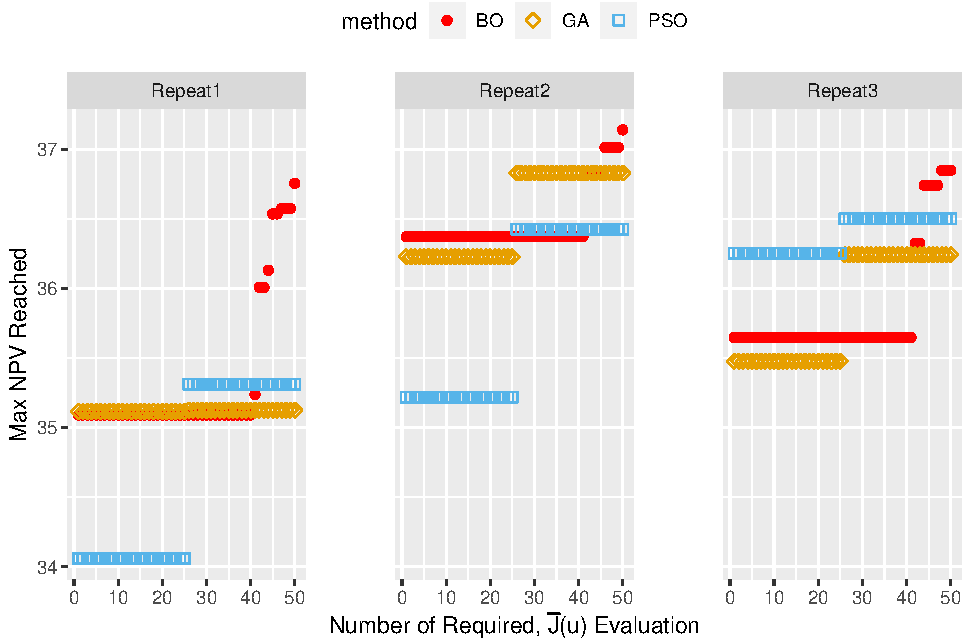
\includegraphics[width=0.9\linewidth]{0_Paper1_main_files/figure-latex/comp-fixbud-1} 

}

\caption{Comparison of GA, PSO and BayesOpt performance at fixed function evaluation budget}\label{fig:comp-fixbud}
\end{figure}

In this work we did not suffice the comparison to only \ref{fig:comp-freebud}. In Figure \ref{fig:comp-freebud} we further allowed the number of \(\overline{J}(u)\) evaluations to 250, while keep the results of BayesOpt to the 50. Meaning that PSO and GA algorithm will enjoy another 8 iterations (\(25\times8=200\)) and then their results, will be compared with BayesOpt from previous section. Figure \ref{fig:comp-freebud} does not convey a single message about performance of these methods. In \ref{tab:comp-tab} median value of three algorithm was compared. The value in second column of \ref{tab:comp-tab} is mean value of each optimization method. (In three repetitions, the maximum achieved NPV is a\textless b\textless c, b was selected). As the \ref{tab:comp-tab} shows, the difference between the NPV value of BayesOpt is almost negligible compared to PSO and GA, while the max NPV in BayesOpt was achieved in 50 \(\overline{J}(u)\) while other two in 250. In this work and optimization setting of the 3D, synthetic reservoir model, BayesOpt reaches same optimal solution, while having computaional complexity of 5X (times) less.

\begin{figure}

{\centering 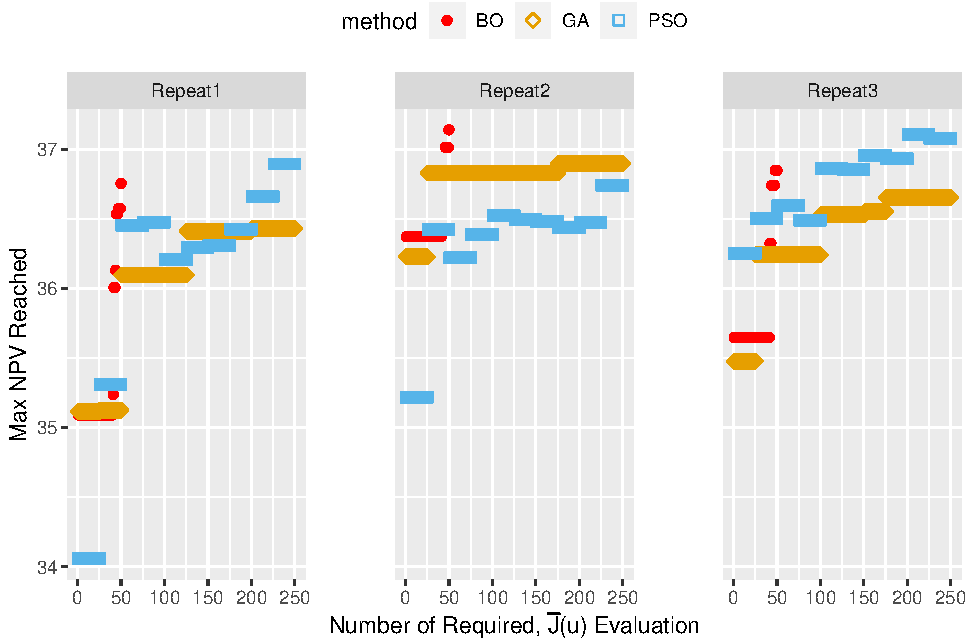
\includegraphics[width=0.9\linewidth]{0_Paper1_main_files/figure-latex/comp-freebud-1} 

}

\caption{Comparison of GA PSO and BayesOpt performance at fixed function evaluation budget}\label{fig:comp-freebud}
\end{figure}

\begin{table}

\caption{\label{tab:comp-tab}Summary table for comparison of GA/PSO and Bayesopt}
\centering
\begin{tabu} to \linewidth {>{\centering}X>{\centering}X>{}c}
\toprule
Optimization Method & Maximum Achieved NPV (median) & $\overline{J}(u)$ Evaluations\\
\midrule
Bayesian Optimization & 36.848 & \cellcolor{blue}{50}\\
Particle Swarm Optimization & 36.894 & \cellcolor{blue}{250}\\
Genetic Alghorithm Optimization & 36.429 & \cellcolor{blue}{250}\\
\bottomrule
\end{tabu}
\end{table}

Comparing the Final Solution \(u\) of the Opt algorithms\ldots(the Median Replication was used)

\begin{center}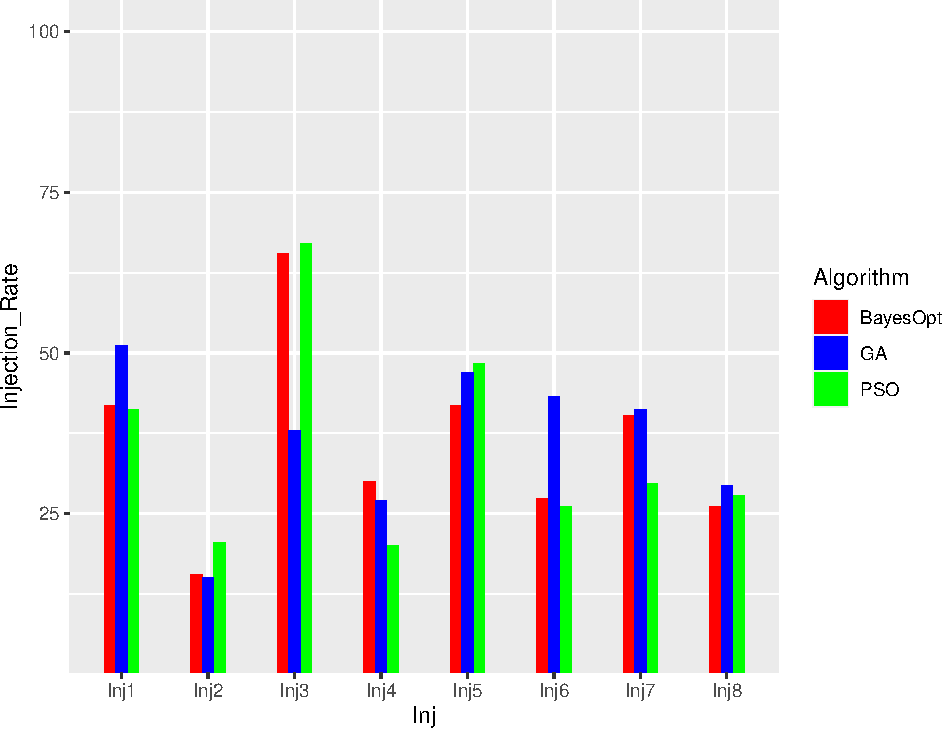
\includegraphics[width=468px]{0_Paper1_main_files/figure-latex/unnamed-chunk-10-1} \end{center}

\newpage

\hypertarget{concluding-remarks}{%
\section{Concluding Remarks}\label{concluding-remarks}}

\newpage

\hypertarget{acknowledgements}{%
\section{Acknowledgements}\label{acknowledgements}}

This work received support from the Research Council of Norway and the companies AkerBP, Wintershall--DEA, Vår Energy, Petrobras, Equinor, Lundin, and Neptune Energy, through the Petromaks--2 DIGIRES project (280473) (\url{http://digires.no}). We acknowledge the access to Eclipse licenses granted by Schlumberger.

\newpage

\hypertarget{references}{%
\section*{References}\label{references}}
\addcontentsline{toc}{section}{References}

\hypertarget{refs}{}
\begin{CSLReferences}{1}{0}
\leavevmode\vadjust pre{\hypertarget{ref-almeida2019}{}}%
Almeida, B.S.G. de, Leite, V.C., 2019. Particle Swarm Optimization: A Powerful Technique for Solving Engineering Problems. IntechOpen.

\leavevmode\vadjust pre{\hypertarget{ref-almeida2007}{}}%
Almeida, L.F., Tupac, Y.J., Pacheco, M.A.C., Vellasco, M.M.B.R., Lazo, J.G.L., 2007. Latin American \& Caribbean Petroleum Engineering Conference. OnePetro. doi:\href{https://doi.org/10.2118/107872-MS}{10.2118/107872-MS}

\leavevmode\vadjust pre{\hypertarget{ref-asadollahi2014}{}}%
Asadollahi, M., Nævdal, G., Dadashpour, M., Kleppe, J., 2014. Production optimization using derivative free methods applied to Brugge field case. Journal of Petroleum Science and Engineering 114, 22--37. doi:\href{https://doi.org/10.1016/j.petrol.2013.12.004}{10.1016/j.petrol.2013.12.004}

\leavevmode\vadjust pre{\hypertarget{ref-chai2021}{}}%
Chai, Z., Nwachukwu, A., Zagayevskiy, Y., Amini, S., Madasu, S., 2021. An integrated closed-loop solution to assisted history matching and field optimization with machine learning techniques. Journal of Petroleum Science and Engineering 198, 108204. doi:\href{https://doi.org/10.1016/j.petrol.2020.108204}{10.1016/j.petrol.2020.108204}

\leavevmode\vadjust pre{\hypertarget{ref-chang2020}{}}%
Chang, Y., Nffivdal, G., Lorentzen, R.J., 2020. SPE Norway Subsurface Conference. SPE, Virtual, p. D021S008R002. doi:\href{https://doi.org/10.2118/200743-MS}{10.2118/200743-MS}

\leavevmode\vadjust pre{\hypertarget{ref-chen2009}{}}%
Chen, Y., Oliver, D.S., Zhang, D., 2009. Efficient ensemble-based closed-loop production optimization. SPE Journal 14, 634--645. doi:\href{https://doi.org/10.2118/112873-PA}{10.2118/112873-PA}

\leavevmode\vadjust pre{\hypertarget{ref-debrito2020}{}}%
de Brito, D.U., Durlofsky, L.J., 2020. Well control optimization using a two-step surrogate treatment. Journal of Petroleum Science and Engineering 187, 106565. doi:\href{https://doi.org/10.1016/j.petrol.2019.106565}{10.1016/j.petrol.2019.106565}

\leavevmode\vadjust pre{\hypertarget{ref-debrito2021}{}}%
de Brito, D.U., Durlofsky, L.J., 2021. Field development optimization using a sequence of surrogate treatments. Computational Geosciences 25, 35--65. doi:\href{https://doi.org/10.1007/s10596-020-09985-y}{10.1007/s10596-020-09985-y}

\leavevmode\vadjust pre{\hypertarget{ref-dennis}{}}%
Dennis, J.E., n.d. A rigorous framework for optimization of expensive functions by surrogates 13.

\leavevmode\vadjust pre{\hypertarget{ref-do2013}{}}%
Do, S.T., Reynolds, A.C., 2013. Theoretical connections between optimization algorithms based on an approximate gradient. Computational Geosciences 17, 959--973. doi:\href{https://doi.org/10.1007/s10596-013-9368-9}{10.1007/s10596-013-9368-9}

\leavevmode\vadjust pre{\hypertarget{ref-eberhart1995}{}}%
Eberhart, R., Kennedy, J., 1995. A new optimizer using particle swarm theory. Ieee, pp. 39--43.

\leavevmode\vadjust pre{\hypertarget{ref-echeverruxedaciaurri2010}{}}%
Echeverría Ciaurri, D., Isebor, O.J., Durlofsky, L.J., 2010. Application of derivative-free methodologies to generally constrained oil production optimization problems. Procedia Computer Science, ICCS 2010 1, 1301--1310. doi:\href{https://doi.org/10.1016/j.procs.2010.04.145}{10.1016/j.procs.2010.04.145}

\leavevmode\vadjust pre{\hypertarget{ref-fonseca2020}{}}%
Fonseca, R.M., Rossa, E.D., Emerick, A.A., Hanea, R.G., Jansen, J.D., 2020. Introduction to the special issue: Overview of OLYMPUS Optimization Benchmark Challenge. Computational Geosciences 24, 1933--1941. doi:\href{https://doi.org/10.1007/s10596-020-10003-4}{10.1007/s10596-020-10003-4}

\leavevmode\vadjust pre{\hypertarget{ref-foroud2016}{}}%
Foroud, T., Seifi, A., 2016. A Guided Pattern Search with a non-intrusive reduced order modeling for oil production optimization: Brugge field case study. Journal of Petroleum Science and Engineering 147, 570--584. doi:\href{https://doi.org/10.1016/j.petrol.2016.09.026}{10.1016/j.petrol.2016.09.026}

\leavevmode\vadjust pre{\hypertarget{ref-forouzanfar2014}{}}%
Forouzanfar, F., Reynolds, A.C., 2014. Joint optimization of number of wells, well locations and controls using a gradient-based algorithm. Chemical Engineering Research and Design 92, 1315--1328.

\leavevmode\vadjust pre{\hypertarget{ref-goldberg1988}{}}%
Goldberg, D.E., Holland, J.H., 1988. Genetic algorithms and machine learning.

\leavevmode\vadjust pre{\hypertarget{ref-harding1998}{}}%
Harding, T.J., Radcliffe, N.J., King, P.R., 1998. Hydrocarbon production scheduling with genetic algorithms. SPE Journal 3, 99--107. doi:\href{https://doi.org/10.2118/36379-PA}{10.2118/36379-PA}

\leavevmode\vadjust pre{\hypertarget{ref-holland1975}{}}%
Holland, J., 1975. Adaptation in natural and artificial systems, university of michigan press, ann arbor,{''}. Cité page 100.

\leavevmode\vadjust pre{\hypertarget{ref-holland1992}{}}%
Holland, J.H., 1992. Adaptation in natural and artificial systems: An introductory analysis with applications to biology, control, and artificial intelligence. MIT press.

\leavevmode\vadjust pre{\hypertarget{ref-hong2017}{}}%
Hong, A.J., Bratvold, R.B., Nævdal, G., 2017. Robust production optimization with capacitance-resistance model as precursor. Computational Geosciences 21, 1423--1442. doi:\href{https://doi.org/10.1007/s10596-017-9666-8}{10.1007/s10596-017-9666-8}

\leavevmode\vadjust pre{\hypertarget{ref-isebor2013}{}}%
Isebor, O.J., Ciaurri, D.E., Durlofsky, L.J., 2013. SPE Reservoir Simulation Symposium. OnePetro. doi:\href{https://doi.org/10.2118/163631-MS}{10.2118/163631-MS}

\leavevmode\vadjust pre{\hypertarget{ref-jansen2014}{}}%
Jansen, J.D., Fonseca, R.M., Kahrobaei, S., Siraj, M.M., Essen, G.M.V., Hof, P.M.J.V. den, 2014. The egg model {\textendash} a geological ensemble for reservoir simulation. Geoscience Data Journal 1, 192--195. doi:\href{https://doi.org/10.1002/gdj3.21}{10.1002/gdj3.21}

\leavevmode\vadjust pre{\hypertarget{ref-jesmani2016}{}}%
Jesmani, M., Bellout, M.C., Hanea, R., Foss, B., 2016. Well placement optimization subject to realistic field development constraints. Computational Geosciences 20, 1185--1209. doi:\href{https://doi.org/10.1007/s10596-016-9584-1}{10.1007/s10596-016-9584-1}

\leavevmode\vadjust pre{\hypertarget{ref-kim2020}{}}%
Kim, J., Yang, H., Choe, J., 2020. Robust optimization of the locations and types of multiple wells using CNN based proxy models. Journal of Petroleum Science and Engineering 193, 107424. doi:\href{https://doi.org/10.1016/j.petrol.2020.107424}{10.1016/j.petrol.2020.107424}

\leavevmode\vadjust pre{\hypertarget{ref-kim2021}{}}%
Kim, Y.D., Durlofsky, L.J., 2021. A Recurrent Neural Network{\textendash}Based Proxy Model for Well-Control Optimization with Nonlinear Output Constraints. SPE Journal 1--21. doi:\href{https://doi.org/10.2118/203980-PA}{10.2118/203980-PA}

\leavevmode\vadjust pre{\hypertarget{ref-li2012}{}}%
Li, L., Jafarpour, B., 2012. A variable-control well placement optimization for improved reservoir development. Computational Geosciences 16, 871--889.

\leavevmode\vadjust pre{\hypertarget{ref-lushpeev2018}{}}%
Lushpeev, V., Margarit, A., 2018. OPTIMIZATION OF OIL FIELD DEVELOPMENT PROCESS BASED ON EXISTING FORECAST MODEL. Journal of Applied Engineering Science 16. doi:\href{https://doi.org/10.5937/jaes16-17218}{10.5937/jaes16-17218}

\leavevmode\vadjust pre{\hypertarget{ref-mitchell1998}{}}%
Mitchell, M., 1998. An introduction to genetic algorithms. MIT press.

\leavevmode\vadjust pre{\hypertarget{ref-muxf8yner2014}{}}%
Møyner, O., Krogstad, S., Lie, K.-A., 2014. The application of flow diagnostics for reservoir management. SPE Journal 20, 306--323. doi:\href{https://doi.org/10.2118/171557-PA}{10.2118/171557-PA}

\leavevmode\vadjust pre{\hypertarget{ref-murphy2022}{}}%
Murphy, K.P., 2022. Probabilistic machine learning: An introduction. MIT Press.

\leavevmode\vadjust pre{\hypertarget{ref-nasir2021}{}}%
Nasir, Y., Volkov, O., Durlofsky, L.J., 2021. A two-stage optimization strategy for large-scale oil field development. Optimization and Engineering. doi:\href{https://doi.org/10.1007/s11081-020-09591-y}{10.1007/s11081-020-09591-y}

\leavevmode\vadjust pre{\hypertarget{ref-nwachukwu2018}{}}%
Nwachukwu, A., Jeong, H., Sun, A., Pyrcz, M., Lake, L.W., 2018. SPE Improved Oil Recovery Conference. OnePetro. doi:\href{https://doi.org/10.2118/190239-MS}{10.2118/190239-MS}

\leavevmode\vadjust pre{\hypertarget{ref-pinto2020}{}}%
Pinto, J.W.O., Tueros, J.A.R., Horowitz, B., da Silva, S.M.B.A., Willmersdorf, R.B., de Oliveira, D.F.B., 2020. Gradient-free strategies to robust well control optimization. Computational Geosciences 24, 1959--1978. doi:\href{https://doi.org/10.1007/s10596-019-09888-7}{10.1007/s10596-019-09888-7}

\leavevmode\vadjust pre{\hypertarget{ref-rasmussen2006}{}}%
Rasmussen, C.E., Williams, C.K.I., 2006. Gaussian processes for machine learning, Adaptive computation and machine learning. MIT Press, Cambridge, Mass.

\leavevmode\vadjust pre{\hypertarget{ref-sarma2005}{}}%
Sarma, P., Aziz, K., Durlofsky, L.J., 2005. SPE Reservoir Simulation Symposium. OnePetro. doi:\href{https://doi.org/10.2118/92864-MS}{10.2118/92864-MS}

\leavevmode\vadjust pre{\hypertarget{ref-scrucca2013}{}}%
Scrucca, L., 2013. GA: A Package for Genetic Algorithms in R. Journal of Statistical Software 53, 1--37. doi:\href{https://doi.org/10.18637/jss.v053.i04}{10.18637/jss.v053.i04}

\leavevmode\vadjust pre{\hypertarget{ref-shahriari2016}{}}%
Shahriari, B., Swersky, K., Wang, Z., Adams, R.P., de Freitas, N., 2016. Taking the human out of the loop: A review of bayesian optimization. Proceedings of the IEEE 104, 148--175. doi:\href{https://doi.org/10.1109/JPROC.2015.2494218}{10.1109/JPROC.2015.2494218}

\leavevmode\vadjust pre{\hypertarget{ref-silva2020}{}}%
Silva, V.L.S., Cardoso, M.A., Oliveira, D.F.B., de Moraes, R.J., 2020. Stochastic optimization strategies applied to the OLYMPUS benchmark. Computational Geosciences 24, 1943--1958. doi:\href{https://doi.org/10.1007/s10596-019-09854-3}{10.1007/s10596-019-09854-3}

\leavevmode\vadjust pre{\hypertarget{ref-stordal2016}{}}%
Stordal, A.S., Szklarz, S.P., Leeuwenburgh, O., 2016. A Theoretical look at Ensemble-Based Optimization in Reservoir Management. Mathematical Geosciences 48, 399--417. doi:\href{https://doi.org/10.1007/s11004-015-9598-6}{10.1007/s11004-015-9598-6}

\leavevmode\vadjust pre{\hypertarget{ref-torczon1997}{}}%
Torczon, V., 1997. On the convergence of pattern search algorithms. SIAM Journal on Optimization 7, 1--25. doi:\href{https://doi.org/10.1137/S1052623493250780}{10.1137/S1052623493250780}

\leavevmode\vadjust pre{\hypertarget{ref-vanessen2009}{}}%
van Essen, G.M., Zandvliet, M.J., Jansen, J.D., 2009. Robust Waterflooding Optimization of Multiple Geological Scenarios. SPE Journal 9.

\leavevmode\vadjust pre{\hypertarget{ref-volkov2018}{}}%
Volkov, O., Bellout, M.C., 2018. Gradient-based constrained well placement optimization. Journal of Petroleum Science and Engineering 171, 1052--1066.

\leavevmode\vadjust pre{\hypertarget{ref-yousef2006}{}}%
Yousef, A.A., 2006. A Capacitance Model To Infer Interwell Connectivity From Production- and Injection-Rate Fluctuations 17.

\leavevmode\vadjust pre{\hypertarget{ref-zhao2015}{}}%
Zhao, H., Kang, Z., Zhang, X., Sun, H., Cao, L., Reynolds, A.C., 2015. SPE Reservoir Simulation Symposium. Society of Petroleum Engineers, Houston, Texas, USA. doi:\href{https://doi.org/10.2118/173213-MS}{10.2118/173213-MS}

\end{CSLReferences}


\end{document}
